\subsection{Finite State Machine - FSM}

\subsubsection{Diagramas de FSM}

Con los diagramas de máquinas de estado (Finite State Machine - FSM) decidimos modelar los comportamientos del sistema que \textbf{requerían sincronización}. Estos comportamientos se representan mediante eventos y estados, y flechas indicando que evento lleva a que estado. Estos eventos pueden realizarse bajo condiciones y modificar el valor de variables predefinidas. También se utilizaron variables de tipo timer que representan a cronómetros (el tiempo de cada timer transcurrirá en el estado que haga referencia a éste). 


Los comportamientos modelados son:
\begin{itemize}
\item El procesamiento de los pedidos de los clientes (creación, modificación, restricciones en las cantidades pedidas, etc).
\item La reserva del stock del depósito en respuesta al pedido de un cliente.
\item El funcionamiento de las alarmas de cada producto en cada depósito.
\item La penalización de los usuarios cuando no reciben un pedido.
\item La actualización del stock luego de un pedido al proveedor.
\end{itemize}


Tres cosas importantes que se deben ver en este modelo son:
\begin{itemize}
\item Cuando un cliente confirma su pedido (mediante ``Realiza un pedido''), el sistema reserva en el depósito el stock necesario para satisfacer dicho pedido y, en caso de no poder satisfacerlo, dicho pedido no es aceptado.
\item Al igual que en el caso de uso ``Modificando pedido'', no se permite que un cliente quite productos o unidades de un producto que ya pidió. Solo se le permite agregar productos o unidades. Esto es así porque los productos del pedido original pudieron ya haber sido cobrados al cliente.
\item Cuando un cliente está en su periodo de penalización, no es capaz de iniciar nuevos pedidos, es decir, el sistema los rechaza.
\end{itemize}

A continuación mostraremos las máquinas de estado realizadas, las cuales se sincronizan todas entre si para dar lugar al comportamiento completo del sistema:

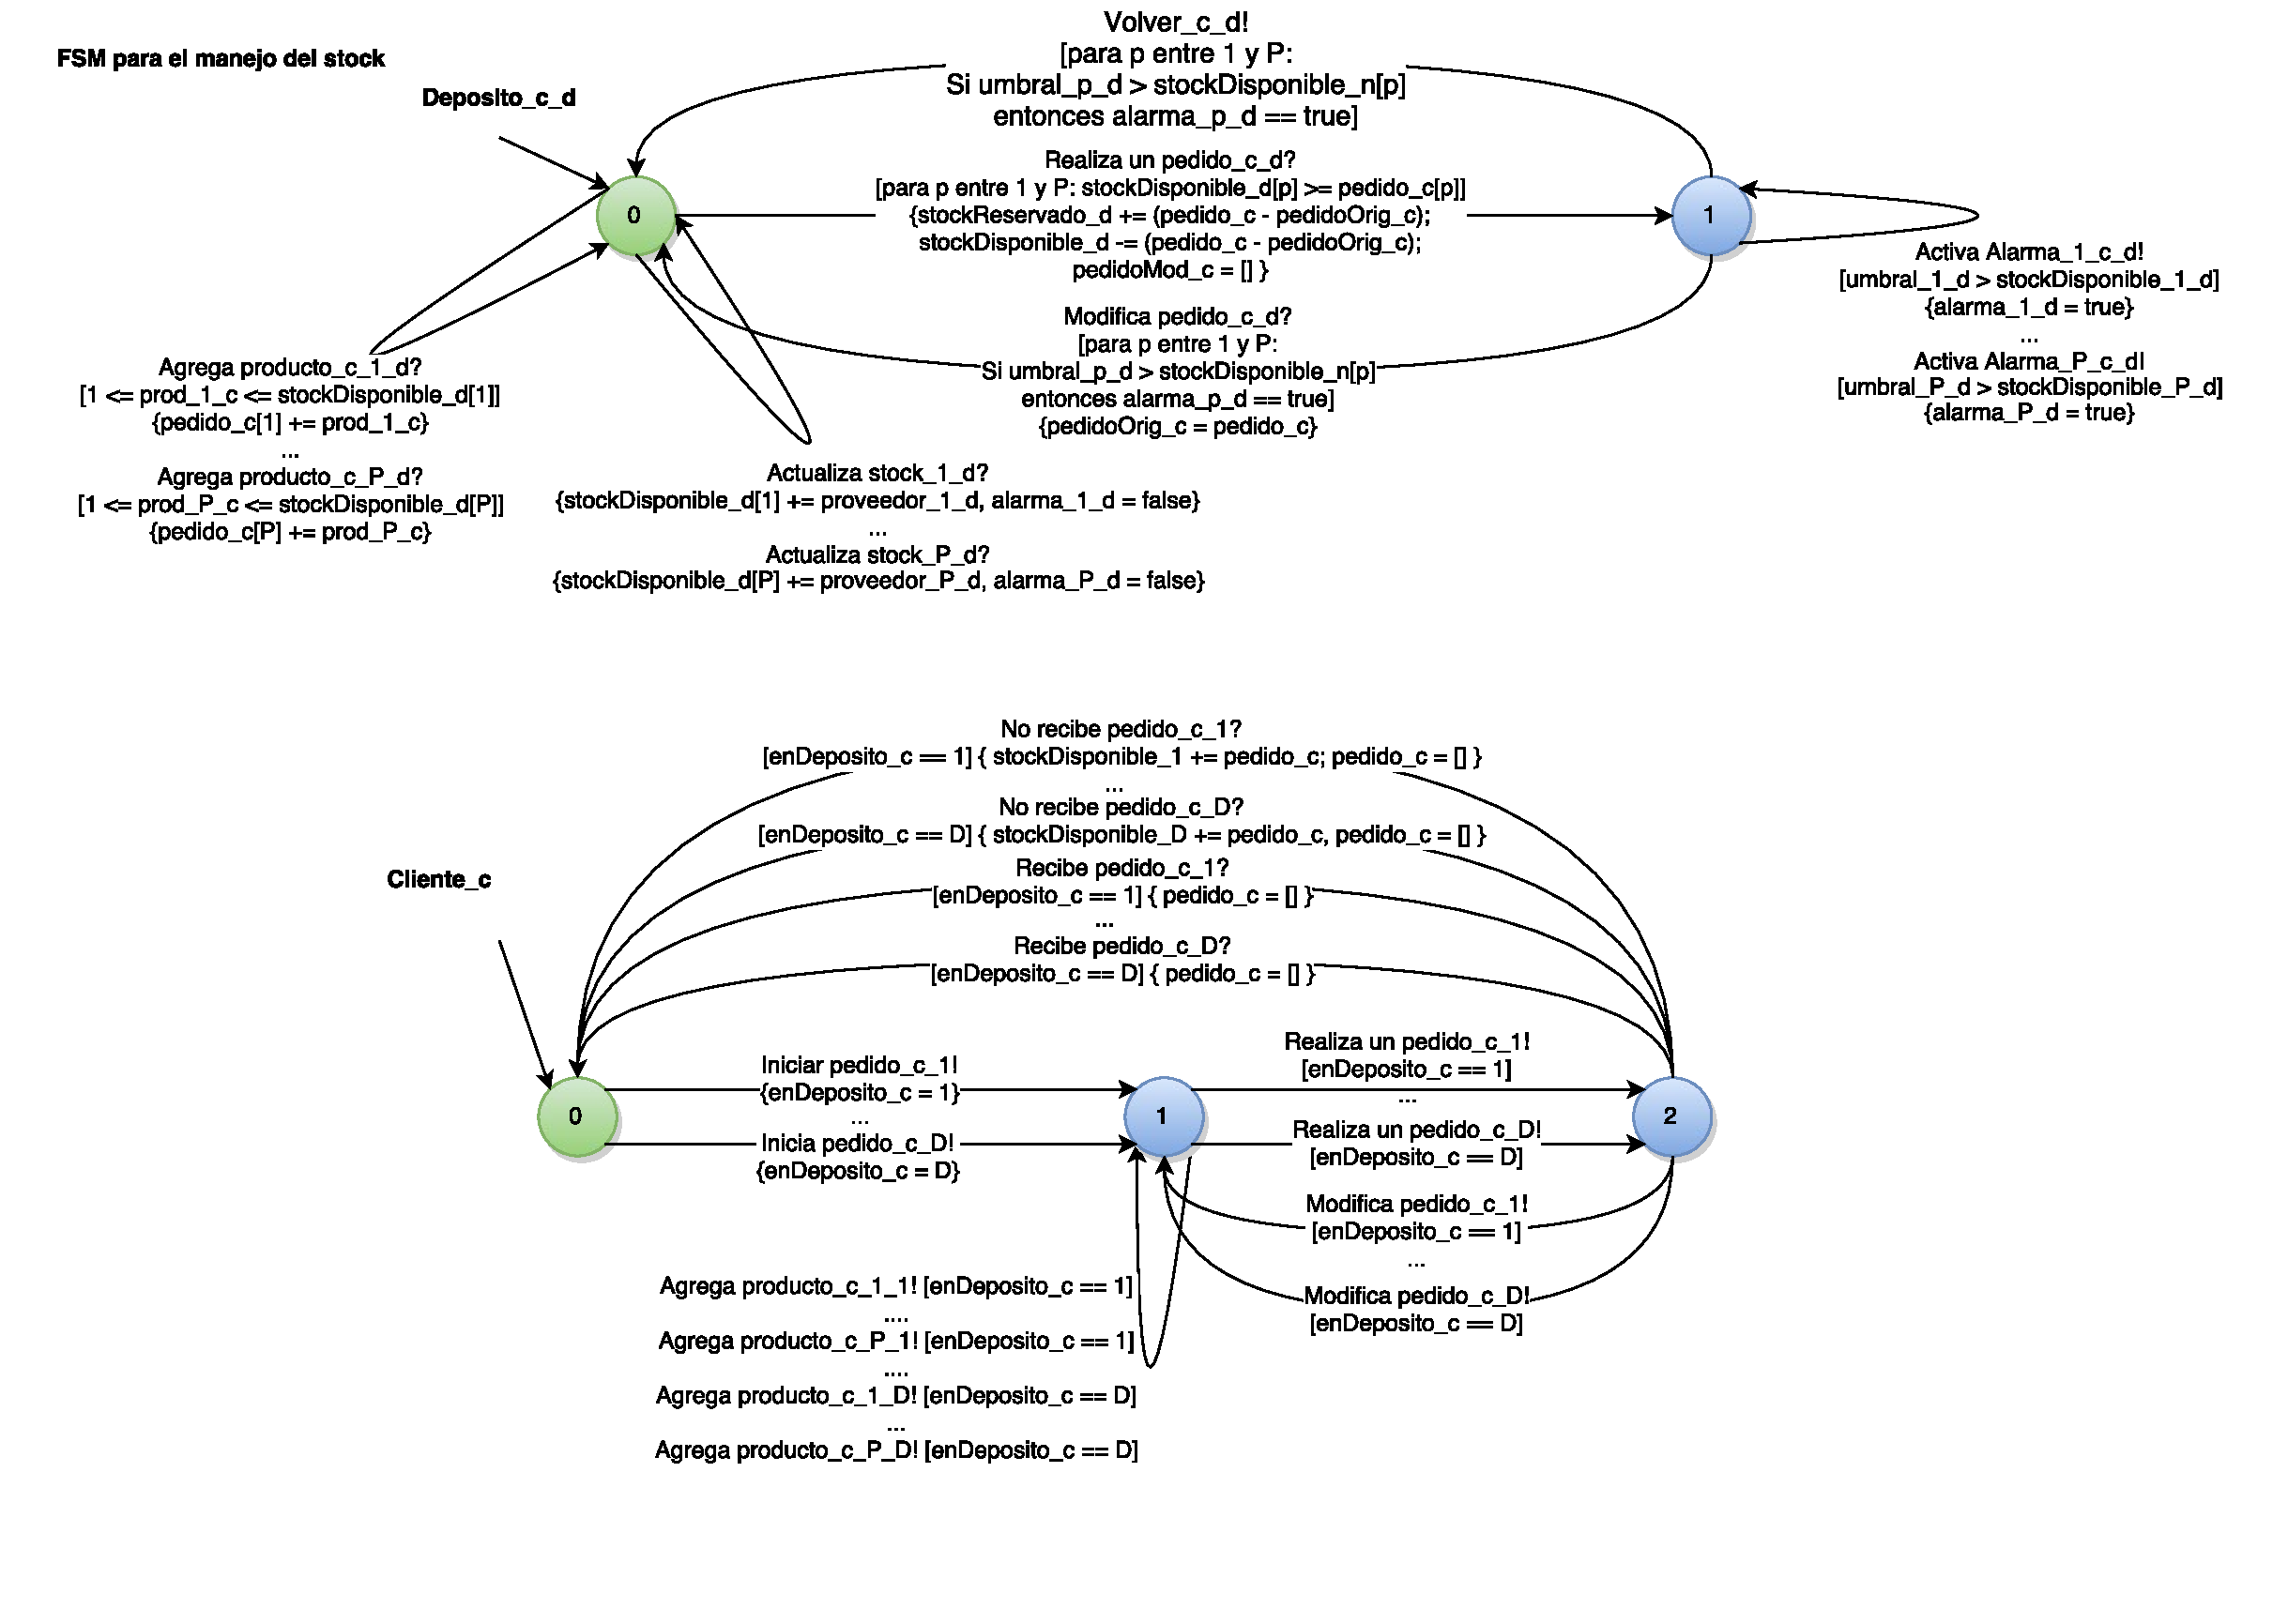
\includegraphics[scale=0.5, angle=90]{secciones/FSM}

\newpage

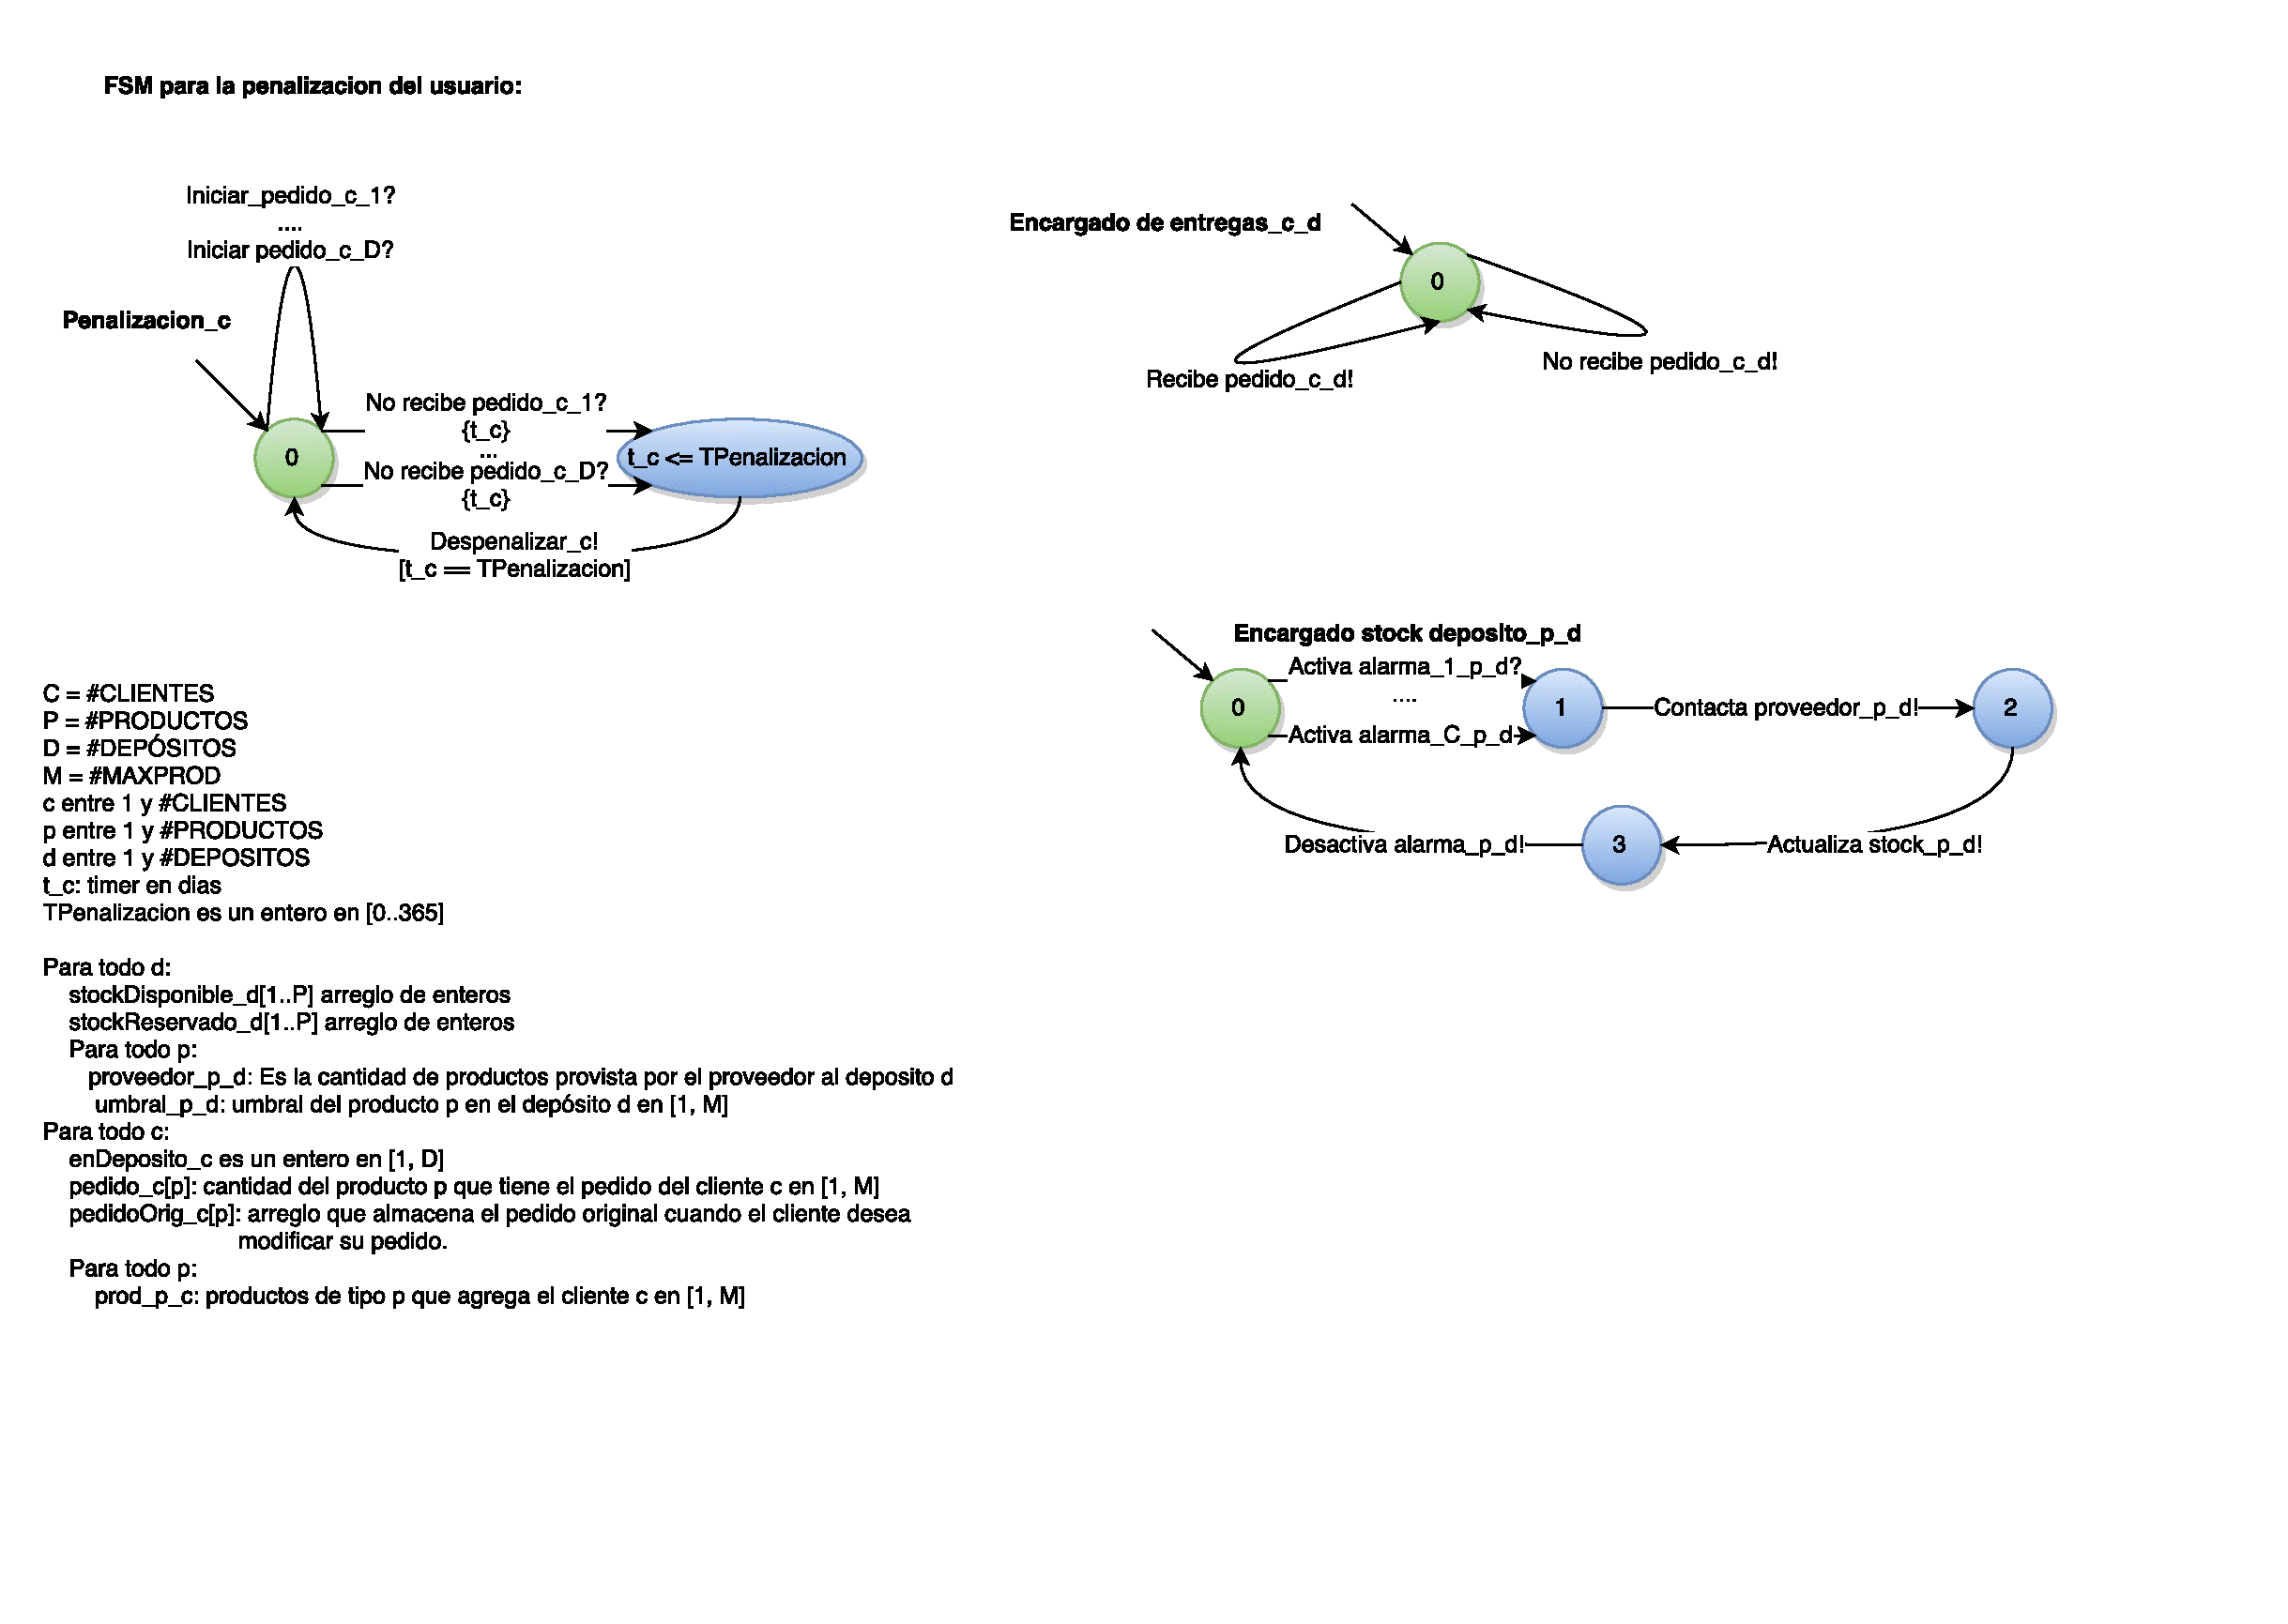
\includegraphics[scale=0.5, angle=90]{secciones/FSM2}

\newpage

El comportamiento del sitio web con respecto a un deposito esta dado por la composición paralela de:
\begin{center}
$Deposito_d$ = $Deposito\_1\_d$ || $Deposito\_2\_d$ || \ldots || $Deposito\_C\_d$.
\end{center}

El comportamiento del sistema de penalización de usuarios esta dado por la composición paralela de:
\begin{center}
$Penalizacion$ = $Penalizacion\_1$ || $Penalizacion_2$ || \ldots || $Penalizacion_C$
\end{center}

El comportamiento del encargado de entregas de un deposito esta dado por la composición paralela de:
\begin{center}
$Encargado\ de\ entregas\_d$ = $Encargado\ de\ entregas\_1\_d$ || $Encargado\ de\ entregas\_2\_d$ || \ldots || $Encargado\ de\ entregas\_C\_d$
\end{center}

El comportamiento del encargado de stock de un deposito esta dado por la composición paralela de:
\begin{center}
$Encargado\ de\ stock\ deposito\_d$ = $Encargado\ de\ stock\ deposito\_1\_d$ || $Encargado\ de\ stock\ deposito\_2\_d$ || \ldots || $Encargado\ de\ stock\ deposito\_P\_d$
\end{center}

El comportamiento completo del sistema esta dado por la composición paralela de:
\begin{center}
$Sistema$ = $Penalizacion$ || $Deposito\_1$ || \ldots || $Deposito\_D$ || $Encargado\ de\ entregas\_1$ || \ldots || $Encargado\ de\ entregas\_D$ || $Encargado\ de\ stock\ deposito\_1$ || \ldots || $Encargado\ de\ stock\ deposito\_D$ || $Cliente\_1$ || \ldots || $Cliente\_C$
\end{center}

\subsubsection{Trazabilidad}
A continuación listamos los requerimientos que se modelan con este diagrama:
\begin{itemize}
\item \textbf{Incrementar stock cuando recibo reposición del proveedor:} en la maquina encargado stock $deposito\_d$, la acción $actualizarStock\_d$
\item \textbf{Los clientes pueden y ver y seleccionar los productos que desean recibir:} maquina $Cliente\_c$, acción $agregaProducto\_c\_p\_d$
\item \textbf{Reservar stock:} maquina $Deposito\_d$, acción $realizaPedido\_c\_d$
\item \textbf{Los productos en falta son filtrado del listado que ve el cliente:} maquina $Deposito\_d$, acción $agregaProducto\_c\_p\_d$
\item \textbf{La cantidad máxima permitida para pedir un producto es igual a la que hay en el deposito:} maquina $Deposito\_d$, acción $agregaProducto\_c\_p\_d$
\item \textbf{Proveedor envía producto:} maquina $EncargadoStockDeposito\_d$, acción $actualizarStock\_d$
\item \textbf{Llevar el conteo en base a los pedidos realizados de cuantos productos quedan:}  array stockDisponible
\item \textbf{Se disparan alarmas cuando la cantidad de productos cae debajo del umbral configurado:} maquina $Deposito_d$, acción $activarAlarma\_p\_d$
\item \textbf{Contactar al proveedor:} $EncargadoStockDeposito\_d$, acción $contactarProveedor\_d$
\item \textbf{Rechazar pedido durante un tiempo:} $Penalizacion\_c$, segundo estado
\item \textbf{Pedido llega a la casa del cliente:} $EncargadoEntregas\_d$, acción $pedidoEnviado\_c\_d$
\end{itemize}

\newpage